数据传输方式包括\textbf{电路交换、报文交换和分组交换}。\\

电路交换、报文交换和分组交换的数据传输方式如图2-4所示。

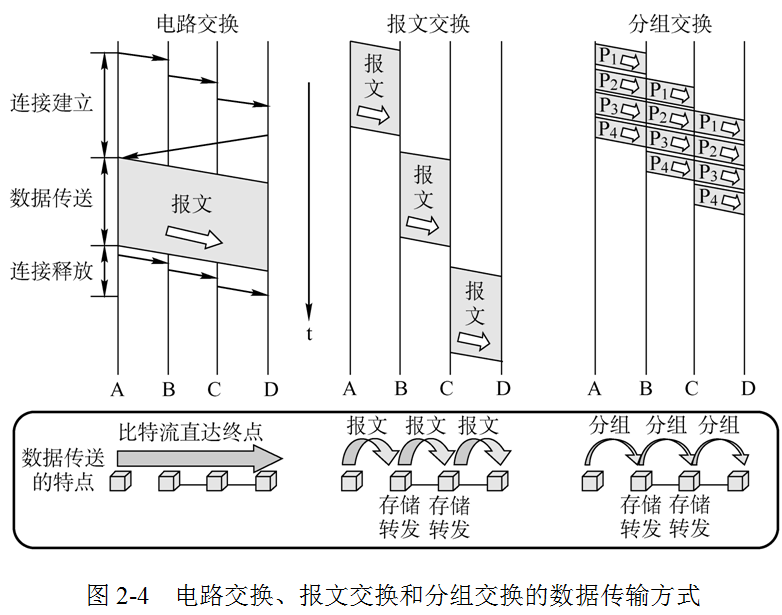
\includegraphics[width=3.12500in,height=2.45833in]{png-jpeg-pics/6065ABA3503AAA626FC3D39C049E76BD.png}

\textbf{{1.电路交换}}

由于电路交换{\textbf{在通信之前要在通信双方之间建立一条被双方独占的物理通路}},因此有以下优缺点。

\textbf{优点:}通信时延小、实时性强、有序传输,并且不同的通信双方拥有不同的信道,不会出现争用物理信道的问题。\\
\textbf{缺点:}建立连接时间长、信道利用率低、缺乏统一标准、灵活性差。

\textbf{{2.报文交换}}

数据交换的单位是\textbf{报文},报文携带有目标地址、源地址等信息。报文交换在交换结点\textbf{{采用存储转发的传输方式}},因而有以下优缺点。

\textbf{优点:}无需建立连接、动态分配线路、可靠性高、线路利用率高、提供多目标服务。\\
\textbf{缺点:}由于数据进入交换结点后要经历存储、转发这一过程,从而\textbf{引起转发时延}(包括接收报文、检验正确性、排队、发送时间等)。报文交换对报文的大小没有限制,这就\textbf{要求网络结点需要有较大的存储缓存空间}。

\textbf{{3.分组交换}}

分组交换\textbf{{仍采用存储转发传输方式}},但将一个长报文先分割为若干个较短的分组,然后把这些分组(携带源、目的地址和编号信息)逐个地发送出去,因此分组交换除了具有报文的优点外,与报文交换相比有以下优缺点。

\textbf{优点:}加速传输、简化了存储管理、减少了出错几率和重发数据量。\\
\textbf{缺点:}存在传输时延、可能出现失序、丢失或重复分组。

\textbf{综上},若要传送的数据量很大,且其传送时间远大于呼叫时间,则采用电路交换较为合适;当端到端的通路由很多段的链路组成时,采用分组交换传送数据较为合适。从提高整个网络的信道利用率上看,报文交换和分组交换优于电路交换,其中分组交换比报文交换的时延小,尤其适合于计算机之间的突发式的数据通信。

\textbf{{4.电路交换与分组交换的特性比较}}

见表2-1。

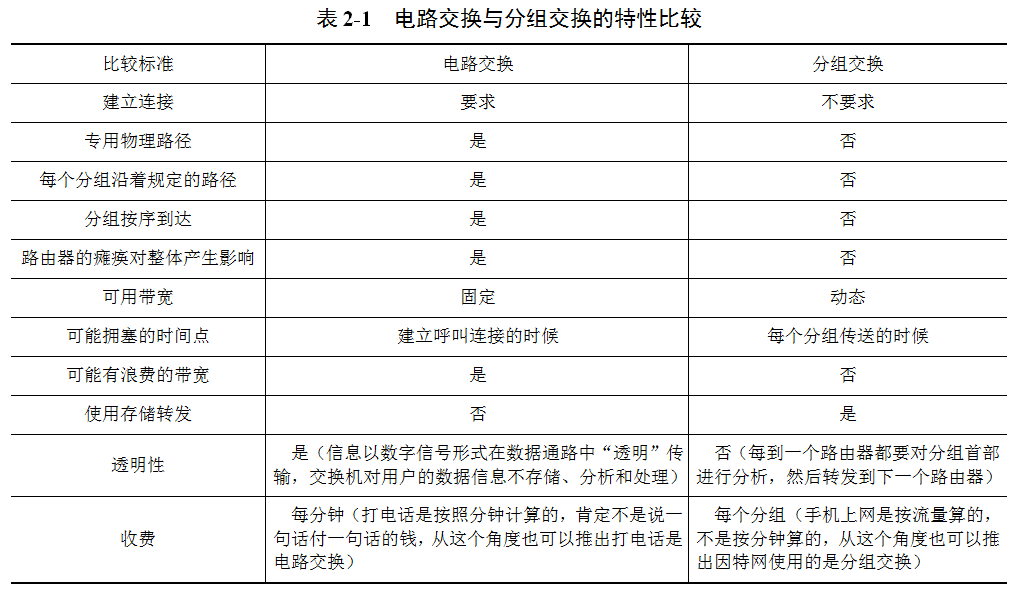
\includegraphics[width=3.33333in,height=1.92708in]{png-jpeg-pics/5C795719AC1A3CA85C9C50184BF417B7.png}
